\documentclass{article}

\usepackage{graphicx}
\usepackage{tikz}
\usepackage{tikzsymbols}
\usetikzlibrary{calc,patterns,shapes.geometric}
\pagestyle{empty}
\usepackage[margin=0pt]{geometry}
\geometry{papersize={14in,12in}}

\def\centerarc[#1](#2)(#3:#4:#5){\draw[#1] ($(#2)+({#5*cos(#3)},{#5*sin(#3)})$) arc (#3:#4:#5);}

\begin{document}
	\begin{figure}
		\centering
		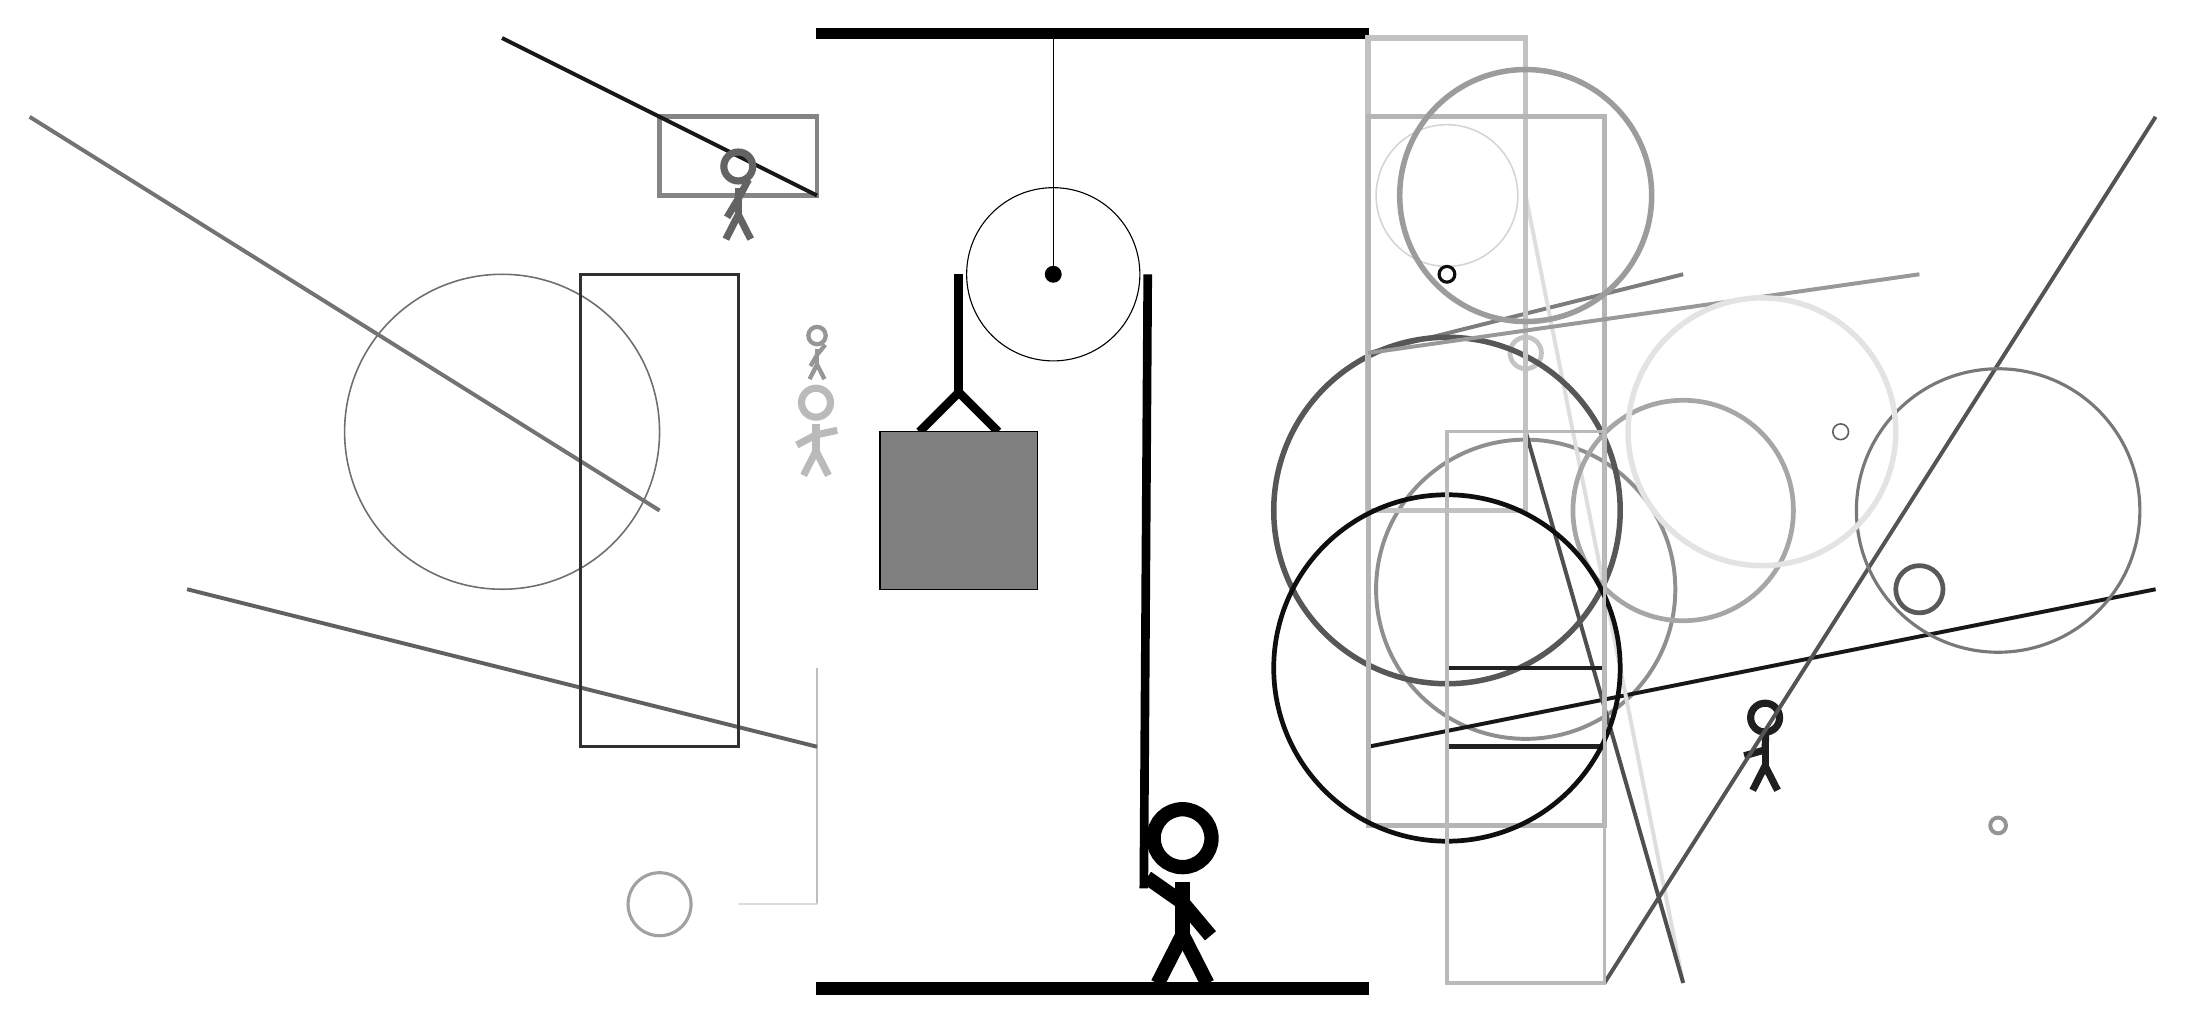
\begin{tikzpicture}
			%%%%% START %%%%%
			
			\draw[fill=black] (-2, 9) rectangle (5, 9.125);
			
			\draw (1, 6) circle (1.1);
			\draw[fill=black] (1, 6) circle (0.1);
			\draw (1, 9) -- (1, 6);
			
			\draw[line width=1.1mm] (-0.7, 4.0) -- (-0.2, 4.5) -- (0.3, 4.0);
			\draw[fill=black!50] (-1.2, 4.0) rectangle (0.8, 2.0);
			
			\draw [line width=0.5mm, color=black!44](7, 2) circle (1.9);
			
			\draw [line width=0.6mm, color=black!23](7, 5) circle (0.2);
			\draw[line width=0.6mm, color=black!48] (-4, 8) rectangle (-2, 7);
			\draw [line width=0.2mm, color=black!17](6, 7) circle (0.9);
			
			\draw[line width=0.5mm, color=black!91](5, 0) -- (15, 2);
			\node[line width=0.7mm, color=black!27] at (-2, 4) {\Strichmaxerl[5][28][12]};
			\draw[line width=0.5mm, color=black!51](5, 5) -- (9, 6);
			
			\draw[line width=0.5mm, color=black!13](9, -3) -- (7, 7);
			\draw[line width=0.2mm, color=black!50] (7, 4) rectangle (7, 6);
			\draw [line width=0.2mm, color=black!63](11, 4) circle (0.1);
			
			\draw [line width=0.2mm, color=black!57](-6, 4) circle (2.0);
			\node[line width=0.4mm, color=black!88] at (10, 0) {\Strichmaxerl[5][16][88]};
			\draw[line width=0.5mm, color=black!69](9, -3) -- (7, 4);
			
			\draw[line width=0.3mm, color=black!26] (-2, 1) rectangle (-2, -2);
			\draw[line width=0.2mm, color=black!14] (-3, -2) rectangle (-2, -2);
			\draw[line width=0.5mm, color=black!62](-2, 0) -- (-10, 2);
			\draw[line width=0.5mm, color=black!67](8, -3) -- (15, 8);
			\draw[line width=0.3mm, color=black!92] (6, 5) rectangle (6, 5);
			\draw [line width=0.4mm, color=black!37](-4, -2) circle (0.4);
			
			\draw [line width=0.6mm, color=black!65](12, 2) circle (0.3);
			\node[line width=0.2mm, color=black!41] at (-2, 5) {\Strichmaxerl[3][60][51]};
			
			\draw [line width=0.5mm, color=black!42](13, -1) circle (0.1);
			
			\draw[line width=0.5mm, color=black!90](-2, 7) -- (-6, 9);
			\draw [line width=0.7mm, color=black!66](6, 3) circle (2.2);
			\draw [line width=0.4mm, color=black!95](6, 6) circle (0.1);
			\draw[line width=0.5mm, color=black!55](-4, 3) -- (-12, 8);
			
			\draw[line width=0.7mm, color=black!24] (5, 9) rectangle (7, 3);
			\draw [line width=0.6mm, color=black!35](9, 3) circle (1.4);
			\draw[line width=0.6mm, color=black!87] (6, 0) rectangle (8, 1);
			\draw[line width=0.6mm, color=black!29] (5, -1) rectangle (8, 8);
			\draw [line width=0.6mm, color=black!94](6, 1) circle (2.2);
			
			\draw[line width=0.4mm, color=black!27] (6, -3) rectangle (8, 4);
			\node[line width=0.3mm, color=black!61] at (-3, 7) {\Strichmaxerl[5][59][62]};
			\draw [line width=0.7mm, color=black!39](7, 7) circle (1.6);
			\draw[line width=0.5mm, color=black!40](5, 5) -- (12, 6);
			\draw [line width=0.4mm, color=black!53](13, 3) circle (1.8);
			\draw[line width=0.4mm, color=black!81] (-3, 6) rectangle (-5, 0);
			
			\draw [line width=0.7mm, color=black!11](10, 4) circle (1.7);
			
			\draw[line width=1.1mm] (-0.2, 6) -- (-0.2, 4.5);
			\centerarc[line width=1.1mm](1, 6)(0:180:1.2000000000000002);
			\draw[line width=1.1mm](2.2, 6) -- (2.15, -1.8);
			
			\node at (2.6, -1.9) {\Strichmaxerl[10][-35][-50]};
			
			\draw[fill=black] (-2, -3) rectangle (5, -3.15);
			
			%%%%% END %%%%%
		\end{tikzpicture}
	\end{figure}	
\end{document}